% =============================================================================
% Project : THE_PHILOSOPHY_OF_VIABILITY
% Book    : Book I — Ontology of Viability
% Book ID : VS.B01
%
% File    : 4_ASSETS/diagrams/VS.B01.P01.C03.S08.SS12.P003.DG01.limits_of_inference_across_ontological_respects.tex
%
% Asset:
%   Diagram DG01 — Limits of Inference Across Ontological Respects
%
% Purpose :
%   To distinguish several ontological respects in which unity
%   and plurality may be examined, and to show that conclusions
%   established in one respect do not automatically transfer
%   to another.
%
% =============================================================================

\begin{figure}[htbp]
\centering

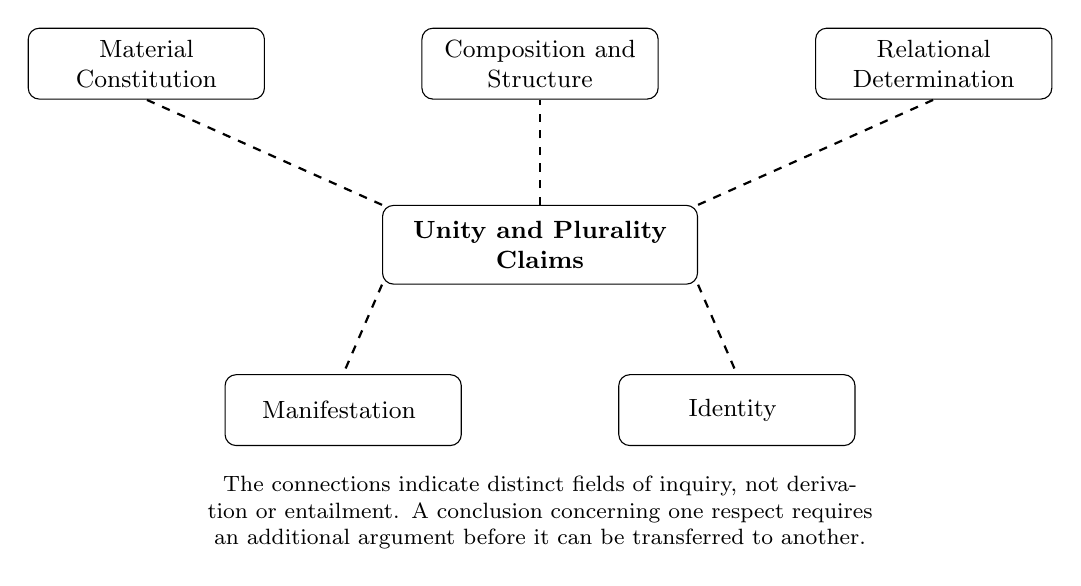
\begin{tikzpicture}[
    respect/.style={
        draw,
        rounded corners,
        align=center,
        minimum width=3.0cm,
        minimum height=0.9cm,
        font=\small
    },
    central/.style={
        draw,
        rounded corners,
        align=center,
        minimum width=4.0cm,
        minimum height=1.0cm,
        font=\small\bfseries
    },
    nonentailment/.style={
        dashed,
        thick,
        -
    }
]

\node[central] (inquiry) at (0,0) {
    Unity and Plurality\\
    Claims
};

\node[respect] (material) at (-5,2.3) {
    Material\\
    Constitution
};

\node[respect] (composition) at (0,2.3) {
    Composition and\\
    Structure
};

\node[respect] (relation) at (5,2.3) {
    Relational\\
    Determination
};

\node[respect] (manifestation) at (-2.5,-2.1) {
    Manifestation
};

\node[respect] (identity) at (2.5,-2.1) {
    Identity
};

\draw[nonentailment] (inquiry.north west) -- (material.south);
\draw[nonentailment] (inquiry.north) -- (composition.south);
\draw[nonentailment] (inquiry.north east) -- (relation.south);
\draw[nonentailment] (inquiry.south west) -- (manifestation.north);
\draw[nonentailment] (inquiry.south east) -- (identity.north);

\node[
    align=center,
    text width=0.92\textwidth,
    font=\footnotesize
] at (0,-3.4) {
    The connections indicate distinct fields of inquiry,
    not derivation or entailment. A conclusion concerning
    one respect requires an additional argument before
    it can be transferred to another.
};

\end{tikzpicture}

\caption{Limits of Inference Across Ontological Respects}
\label{fig:limits-of-inference-across-ontological-respects}
\end{figure}

% =============================================================================
% END OF DIAGRAM DG01
% =============================================================================